% ============================================================
% Chapter 5: Results and Discussion
% ============================================================
\chapter{Results and Discussion}
\label{chap:results}

This chapter presents and analyses the results of the verification and validation (V\&V) activities described in~\Cref{chap:testing}. It first evaluates to what extent functional equivalence with the legacy anti-skid test-diagnosis module~\cite{rexroth1992wsp} was achieved, layer by layer and in a summary table (\Cref{sec:equivalence_outcomes}). It then classifies the integration defects discovered on the way and what they reveal about the two layers (\Cref{sec:integration_defects}), describes the causes of the two defects in the diagnostic path and the fix applied (\Cref{sec:diagnostic_resolution}), discusses the relation to the targeted safety standards (\Cref{sec:safety_compliance}), and closes with risks and limitations (\Cref{sec:results_discussion_risk}).

% ------------------------------------------------------------
\section{Functional Equivalence and Test Outcomes}
\label{sec:equivalence_outcomes}

The central goal was to demonstrate that the retrofitted hardware replicates the behaviour of the original test-diagnosis module. Bringing the rebuilt unit to a testable state required overcoming the hardware and software integration challenges described in~\Cref{subsec:hardware_challenges}.

\subsection{Layer 1: Component and Interface Test Results}
\label{subsec:fpga_interface_results}

Component-level verification is meant to isolate issues at the hardware and \gls{hdl} level before system integration; here it did not isolate the \gls{nvram} enable defect (B1, \Cref{tab:bug_taxonomy}). The Layer~1 results are:
\begin{itemize}
	\item \textbf{\gls{vhdl} Simulation:} The archived simulation of the inherited design (testbench \texttt{tb\_testDiagnose.vhd}, September 2023) completed without errors although the byte-low enable \texttt{NVRAM\_ble} was held high (\Cref{sec:app_vhdl_testbenches}); the testbench contains no assertions. Its behavioural model of the \gls{nvram} reads and writes on chip enable, output enable and write enable only, and the testbench leaves \texttt{NVRAM\_ble} unconnected (\texttt{tb\_testDiagnose.vhd}, lines 233 and 276--295), so the simulation could not show the defect at all: its escape was a gap of the verification environment. Because the emulated controller uses only the lower data byte of the 16-bit \texttt{CY14B104NA}, this disabled the non-volatile fault memory. Leyer's dedicated \gls{nvram} test designs had stored and recalled data correctly on the prototype~\cite[Sec.~4.4]{leyer2023}; the defect lay in the top-level design. The follow-on team observed its symptoms while testing the rebuilt unit on the fixture: the unit did not respond to the fixture's tests, the Lösch function had no effect and the STW button showed non-existent codes. While debugging, they found \texttt{NVRAM\_ble} held high; driving it permanently low corrected the defect~\cite[pp.~14--15]{savchuk2025}. Leyer's simulations of the complete design had shown the boot sequence, the start of the self-test, the storage of an error condition and the STW read-out as intended~\cite[Sec.~5.1]{leyer2023}; no simulation after the correction of the defect is archived.
	\item \textbf{\gls{jtag} and Pin Checks:} On the Rev~0.0 prototype, Leyer read the device identification (\texttt{A3P1000}) and programmed and verified the bitstream over \gls{jtag}, and he checked every used pin with a toggle test design and a multimeter. After a visual inspection had found two cold solder joints, he programmed the Flash~\gls{rom} through the boundary-scan cells of the \gls{fpga} with \texttt{urjtag}~\cite[Sec.~4.1--4.3]{leyer2023}. In the follow-on work, the processor of the rebuilt unit did not respond to reset and did not fetch from the Flash~\gls{rom} although supply and clock were present, checked with an oscilloscope. While testing, the team noticed four poorly soldered \gls{fpga} pins, and then about 40 further pins had to be re-soldered~\cite[p.~13]{savchuk2025}. The follow-on report does not mention boundary scan for this rework.
	\item \textbf{Hardware Timing Measurements:} The follow-on report's only statement on the watchdog, that it worked and reset the processor, refers to the first debugging step, before the \gls{fpga} pins were re-soldered, in which the team also found that the processor did not respond to the reset signal~\cite[p.~13]{savchuk2025}. No observation of the watchdog after the re-soldering is documented. The frequency sweep, designed to cover \SI{850}{\hertz} to \SI{1550}{\hertz} (\Cref{eq:sweep}), was checked by Leyer against the original board on the Rev~0.0 prototype~\cite[Sec.~4.10]{leyer2023} and is not documented on the rebuilt unit. The captures reproduced in this report were taken by Leyer on the inherited Rev~0.0 prototype in 2023~\cite{leyer2023}. They show the watchdog reset test (\Cref{fig:watchdog_reaction}), in which a test design services the watchdog for about five seconds and then withholds service so that the external watchdog has to reset the controller, and the comparison of the sweep of the original board with that of the \gls{fpga} emulation (\Cref{fig:sweep_comparison}). They document the measurement method. Only for the sweep was the original board measured as a reference; the original watchdog could not be observed, because it acts only when the software or the controller fails~\cite[Sec.~4.6]{leyer2023}. Both captures are analysed below.
\end{itemize}

The Layer~1 results show the limits of this simulation: its model of an external device did not cover every control input, so it passed a design that did not work on the board, and tests and inspection on the hardware were needed as well, particularly on a prototype.

\subsubsection{Watchdog Timing}

Leyer expected the reset line to be pulled low every \SI{1.2}{\second} and reported that the observations on the prototype showed the expected behaviour~\cite[Sec.~4.6]{leyer2023}. He himself, however, doubted the \SI{1.2}{\second}: the original schematic shows \SI{1}{\micro\farad} for the capacitor of the watchdog clock, which measured \SI{100}{\nano\farad}, and the prototype took over \SI{470}{\nano\farad} in parallel with \SI{100}{\nano\farad} from the comparator card; perhaps the \SI{470}{\nano\farad} capacitor would have to be removed~\cite[Sec.~4.6]{leyer2023}. \Cref{tab:bom} lists it as \texttt{C13} on the Upper Board; whether it belongs there is open.

Leyer measured the period of the watchdog clock on the prototype as \SI{180}{\milli\second}, and the most significant bit of the counter pulls the reset line low~\cite[Sec.~4.6]{leyer2023}. In the Rev~1.0 schematic this is the output Q4 of the \gls{bcd} counter \texttt{Y5} (pin \texttt{Q3} in the Eagle library), which drives the transistor \texttt{Q1} through \texttt{D1} and \texttt{R5} (\Cref{fig:schematic_sheet1}). According to its datasheet among the project's files, the counter, enabled here, advances on each rising edge of its clock and is cleared by a high level at its reset input. Q4 goes high at the count of eight, so the reset follows seven to eight clock periods after the last service pulse, about \SIrange{1.3}{1.4}{\second} at \SI{180}{\milli\second}, and while service stays withheld it lasts two periods and recurs every ten. Read from \Cref{fig:watchdog_reaction}, the first reset follows about \SI{1.2}{\second} after the service stops, and resets of about \SI{0.3}{\second} recur about \SI{1.6}{\second} apart; these are approximate readings of a photograph of the screen, and they fit this decoding with a clock period somewhat below \SI{180}{\milli\second}. The \SI{1.2}{\second} Leyer expected is thus the time to the first reset, not the interval between resets. A design value of the clock period has not been derived from the timing components (\texttt{R1}, \texttt{C7} and \texttt{C13}, \Cref{fig:schematic_sheet1}): a derivation would need the threshold voltages of the Schmitt-trigger inputs of the oscillator \texttt{CD40106} at the supply voltage of the circuit, which the sources of this report do not give, and the timing capacitance, which depends on whether \texttt{C13} belongs there.

The reset line has no pull-up resistor in the Rev~1.0 schematic. Leyer advised adding one or enabling the pull-up of the \gls{fpga} pin, which the prototype used~\cite[Sec.~9.2]{leyer2023}. The pin report of the design \path{TestDiagnose_new} of 7~September 2023 shows that pull-up enabled on \path{reset_n}, while the report of the simulated design \path{TestDiagnose} of 4~September 2023 shows none; whether the design of the rebuilt unit enables it is not documented.

\subsubsection{Frequency Sweep}

\begin{figure}[tb]
	\centering
	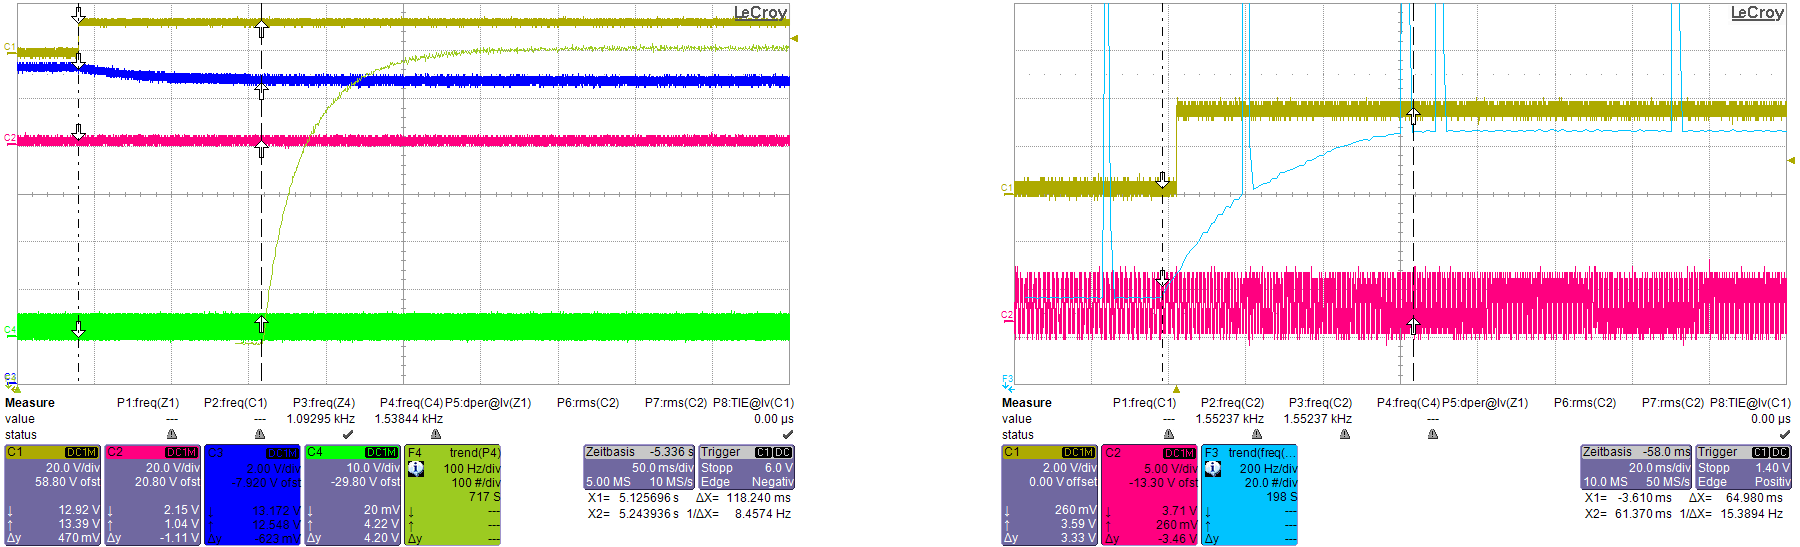
\includegraphics[width=\textwidth]{sweep/comp_upsweep.png}\\[1ex]
	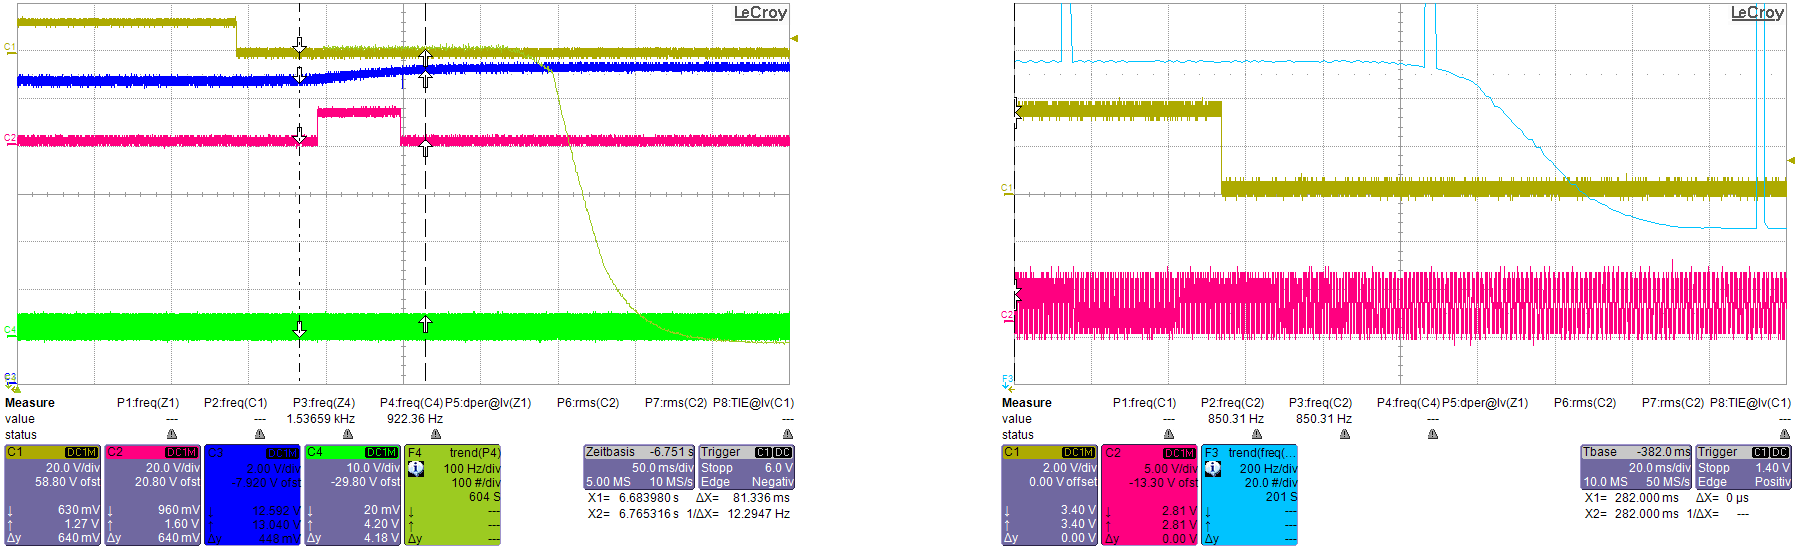
\includegraphics[width=\textwidth]{sweep/comp_downsweep.png}
	\caption[Frequency Sweep: Original Board and FPGA Emulation]{Frequency sweep of the original board (left capture of each pair) and of the \gls{fpga} emulation (right capture), recorded by Leyer on the inherited Rev~0.0 prototype in July~2023. Top: rising sweep; bottom: falling sweep. The thin lines are the oscilloscope's trends of the frequency measurement: they plot its successive values, 100 per division for the original board and 20 for the emulation, so their horizontal axis is not the time base of the traces, although Leyer describes them as the change of frequency over time~\cite[Sec.~4.10]{leyer2023}. The readouts are given in \Cref{tab:sweep_readouts}. Reproduced from~\cite[Figs.~11 and~12]{leyer2023}.}
	\label{fig:sweep_comparison}
\end{figure}

\Cref{tab:sweep_readouts} gives the readouts of the sweep captures. Leyer reports that the end frequencies of \SI{850}{\hertz} and \SI{1550}{\hertz} and the duration of the sweep were checked against the original board and showed the correct values, but gives no values~\cite[Sec.~4.10]{leyer2023}. Read from the captures, the frequency readouts of the original board are \SI{1538.44}{\hertz} in the rising and \SI{922.36}{\hertz} in the falling sweep, those of the emulation \SI{1552.37}{\hertz} and \SI{850.31}{\hertz}. For the self-test of the original test card, the fixture report gives a frequency change from \SI{1540}{\hertz} to \SI{920}{\hertz}~\cite[Sec.~5.1.5]{dolata2023}, in line with the original board's readouts, while the emulation's sweep is designed for \SIrange{849.9}{1549.6}{\hertz} (\Cref{eq:sweep}). The captures do not show what the readouts were measured over, and most of them carry a warning symbol of the oscilloscope. Further captures of the original board in the folder \texttt{Analyse} of Leyer's digital appendix~\cite{leyer2023}, however, read \SI{919.69}{\hertz} (\texttt{ss4.png}), \SI{920.81}{\hertz} (\texttt{ss9.png}) and \SI{920.80}{\hertz} and \SI{921.80}{\hertz} (\texttt{ss34.png}) at the low end. The raw export of the window of \texttt{ss34.png} (\path{C4Signal_red00000.csv}) shows a steady frequency: its 459 periods, evaluated for this report, lie between \SI{916}{\hertz} and \SI{926}{\hertz}, about \SI{920}{\hertz} on average. The periods were taken between consecutive rising crossings of the midpoint between the signal's extremes (\SI{2.12}{\volt}), at the resolution of one sample (\SI{4}{\micro\second}) and with a hysteresis of \SI{0.5}{\volt}. The low end of the original board is therefore about \SI{920}{\hertz}, about \SI{70}{\hertz} above that of the emulation. Leyer's analysis note in the same folder gives \SI{850}{\hertz} as the intended value (\texttt{Widerstände Sweep Counter.txt}); whether \SI{920}{\hertz} is the design value of the original circuit or a drift of this board is open. This report does not record whether Leyer's captures and the fixture report's values for the original test card come from the same unit; if they came from two units, a drift common to both would be less likely, but as it stands the agreement of the two values does not settle the question.

The duration differs as well, as far as the sources allow a comparison. The emulation's rising sweep reaches its end value after about \SI{52}{\milli\second} and its falling sweep after about \SI{102}{\milli\second} (\Cref{sec:fpga_core_details}); its falling table reaches about \SI{920}{\hertz} after 33 steps, about \SI{55}{\milli\second}. For the original test card, the fixture report gives about \SI{180}{\milli\second} for the frequency changes, which its capture reads with cursors as \SI{183.186}{\milli\second}~\cite[Sec.~5.2, Fig.~3]{dolata2023}. The cursor spacings of Leyer's captures (\Cref{tab:sweep_readouts}) cannot be set against these figures, for the reason given with \Cref{tab:sweep_readouts}. Because the sweep simulates a misbehaviour that the axle cards are to recognise as sliding~\cite[Sec.~2.9]{leyer2023}, its duration and slope may matter as much as its end frequencies; the sources do not say which of them the axle cards evaluate. Both points concern the original board rather than the emulation: the emulation's end frequencies and durations follow from its tables and clock dividers, so a measurement of the rebuilt unit would be expected to show these design values if its \gls{fpga} design contains this generator. Settling the low end and the duration of the original's sweep needs a re-measurement of the original board or a check of its sweep circuit; both are open (\Cref{tab:evidence_state}).

\begin{table}[htbp]
	\centering
	\caption[Readouts of the Sweep Captures]{Readouts of the sweep captures of \Cref{fig:sweep_comparison}, read from the archived images, not measured again. P2 to P4 are the measurement parameters as the oscilloscope labels them; what the cursors mark is not documented.}
	\label{tab:sweep_readouts}
	\small
	\begin{tabular}{@{}lll@{}}
		\toprule
		Readout & Original board (left) & \gls{fpga} emulation (right) \\
		\midrule
		Rising sweep: frequency of the channel & \SI{1538.44}{\hertz} (P4) & \SI{1552.37}{\hertz} (P2, P3) \\
		Rising sweep: frequency of the zoomed trace & \SI{1092.95}{\hertz} (P3) & -- \\
		Rising sweep: cursor spacing & \SI{118.240}{\milli\second} & \SI{64.980}{\milli\second} \\
		Falling sweep: frequency of the channel & \SI{922.36}{\hertz} (P4) & \SI{850.31}{\hertz} (P2, P3) \\
		Falling sweep: frequency of the zoomed trace & \SI{1536.59}{\hertz} (P3) & -- \\
		Falling sweep: cursor spacing & \SI{81.336}{\milli\second} & 0 (cursors coincide) \\
		Time base & \SI{50}{\milli\second}/div & \SI{20}{\milli\second}/div \\
		\bottomrule
	\end{tabular}
\end{table}

\subsection{Layer 2: System-Level Test Results}
\label{subsec:system_scenario_results}

In this method, fixture-based testing is the decisive check of functional equivalence. Before the rebuilt unit could be tested, the follow-on team had to make the fixture's firmware debuggable and correct its state machine~\cite[p.~10]{savchuk2025}. On the rebuilt unit the Layer~2 evidence is their report; no fixture log was archived:
\begin{itemize}
	\item \textbf{Fault Memory Cycle:} The legacy diagnosis table~\cite[Blatt~20/25]{rexroth1992wsp} lists, for each of the four axle cards, codes for a sensor fault, a valve short circuit, a valve wire break and a monitoring timeout, and codes for the computer cards 01 to 05. Before the rebuilt unit was tested, the follow-on team had revised the PC software of the fixture so that tests setting two or three pins at once could run~\cite[pp.~10--11]{savchuk2025}. After the \gls{nvram} enable defect (B1) had been corrected, the two-pin tests still aborted, which the team attributed to the PC software~\cite[p.~14]{savchuk2025}. The team then ran the fixture's full suite, which it reports as successful, and a selection of 19 test cases; the expected codes were observed on the displays, but the fixture's camera could not read them~\cite[p.~15]{savchuk2025}. The follow-on report does not say how the abort of the two-pin tests was resolved before these runs. No test log of these runs is part of the archived material. Which fault codes these runs covered is not recorded here. For the sensor faults, \enquote{expected} means the fixture's display code, 31 for axle card~3, where \Cref{tab:requirement_basis} gives 03 (note~b), so for these cases the observation cannot be read as conformity with that table.
	\item \textbf{Self-Test:} The execution of the legacy self-test on the rebuilt unit is not documented. Leyer's simulation showed the start of the self-test sequence as intended~\cite[Sec.~5.1.2]{leyer2023}. The fixture firmware used in the follow-on runs had gained a self-test function~\cite[p.~12]{savchuk2025}; the follow-on report says neither what it tests nor whether those runs used it.
	\item \textbf{User Interface Equivalence:} STW and Lösch are part of the fixture's test sequence~\cite{dolata2023}, and the Lösch function worked after the correction of B1~\cite[p.~14]{savchuk2025}; for the Test and Tür/V buttons no result on the rebuilt unit is documented.
	\item \textbf{Power-Cycle Stability:} No run with power cycles on the rebuilt unit is recorded.
	\item \textbf{\gls{stm32} Diagnostics Logging:} Both defects of the diagnostic path (B4, B5) were open in August 2025~\cite[pp.~19--22]{savchuk2025}; a fix of the firmware of 2023, described in \Cref{sec:diagnostic_resolution}, was applied afterwards; the evidence after it is given in \Cref{tab:evidence_state}.
\end{itemize}

\Cref{tab:results_summary} summarises the verification activities by layer, with the item tested, the date and the source of each result.

% p: with its notes the table is too tall for the top of a text page, and without p it
% held back every later table of the chapter until the chapter ended
\begin{table}[htbp]
	\centering
	\caption[Summary of Verification Results]{Summary of verification results across both layers, with the item tested, the date and the source of each result.}
	\label{tab:results_summary}
	\small
	\setlength{\tabcolsep}{4pt}
	\begin{tabular}{@{}>{\raggedright\arraybackslash}p{0.25\textwidth} l >{\raggedright\arraybackslash}p{0.2\textwidth} >{\raggedright\arraybackslash}p{0.09\textwidth} >{\raggedright\arraybackslash}p{0.13\textwidth} >{\raggedright\arraybackslash}p{0.16\textwidth}@{}}
		\toprule
		Test category & Layer & Item tested & Date & Source & Result \\
		\midrule
		Design simulation in ModelSim (boot, error storage) & L1 & Design of 2023 & 2023 & \cite[Sec.~5.1]{leyer2023} & Pass$^{a}$ \\
		Flash and \gls{nvram} test designs & L1 & Rev~0.0 prototype & 2023 & \cite[Sec.~4.3--4.4]{leyer2023} & Pass \\
		\gls{jtag} ID and programming & L1 & Rev~0.0 prototype & 2023 & \cite[Sec.~4.1]{leyer2023} & Pass \\
		Watchdog reaction & L1 & Rev~0.0 prototype & Aug.\ 2023 & \cite[Sec.~4.6]{leyer2023} & Observed$^{b}$ \\
		Watchdog reaction & L1 & Rebuilt unit, before re-soldering & 2025 & \cite[p.~13]{savchuk2025} & Before rework$^{b}$ \\
		Frequency sweep & L1 & Rev~0.0 prototype and original board & July 2023 & \cite[Sec.~4.10]{leyer2023} & Observed$^{b}$ \\
		Frequency sweep & L1 & Rebuilt unit & -- & -- & Not documented \\
		Fault codes & L2 & Rebuilt unit$^{f}$ & 2025 & \cite[p.~15]{savchuk2025} & Observed$^{c}$ \\
		Operator buttons STW, Lösch & L2 & Rebuilt unit$^{f}$ & 2025 & \cite[pp.~14--15]{savchuk2025} & Observed$^{c}$ \\
		Operator buttons Test, Tür/V & L2 & Rebuilt unit & -- & -- & Not documented \\
		Self-test & L2 & Rebuilt unit & -- & -- & Not documented \\
		Power-cycle stability & L2 & Rebuilt unit & -- & -- & Not documented \\
		Diagnostic \gls{spi} frame & L2 & Rebuilt unit$^{f}$ & -- & -- & Fix applied$^{d}$ \\
		\gls{sd}~card logging & L2 & Rebuilt unit$^{f}$ & -- & -- & Fix applied$^{e}$ \\
		\bottomrule
	\end{tabular}

	\medskip
	\begin{minipage}{0.95\textwidth}
		\footnotesize
		$^{a}$The archived simulation could not detect defect~B1, because its \gls{nvram} model ignores the byte-low enable (\Cref{subsec:fpga_interface_results}).\\
		$^{b}$The archived oscilloscope captures (\Cref{fig:watchdog_reaction,fig:sweep_comparison}) were taken by Leyer on the inherited Rev~0.0 prototype, the sweep also on the original board; the readouts of the sweep are given in \Cref{tab:sweep_readouts}. The cursor readout in~\Cref{fig:watchdog_reaction} measures no watchdog parameter; the timing read from the capture, and Leyer's doubts about it, are given in \Cref{subsec:fpga_interface_results}; unlike the sweep, the watchdog has no capture of the original board as a reference~\cite[Sec.~4.6]{leyer2023}. On the rebuilt unit, the follow-on report's only statement on the watchdog refers to the state before the re-soldering of the \gls{fpga} pins (\Cref{subsec:fpga_interface_results}).\\
		$^{c}$Observed during the follow-on runs (full suite and 19 selected cases); the fixture's camera could not read the displays (\Cref{tab:evidence_state}).\\
		$^{d}$Truncated to 16~bits in the inherited firmware; in 2025 the third byte was also found corrupted in simulation (defect~B5). A fix was applied to the receiver of 2023; whether the transmitter was changed is not documented.\\
		$^{e}$The logging froze with the follow-on firmware of 2025; frames were overrun in the firmware of 2023, to which a fix was applied (defect~B4). For the evidence after the fix of this row and the row above, see \Cref{tab:evidence_state}.\\
		$^{f}$Configuration not documented: the follow-on report names the~\gls{fpga} design of the rebuilt unit only as the new software of the test card, without a version or checksum, and does not say which firmware ran on its \gls{stm32} Diagnostics Board~\cite[p.~15]{savchuk2025} (\Cref{sec:diagnostic_resolution}).
	\end{minipage}
\end{table}

\subsection{State of the Evidence}
\label{subsec:equivalence_discussion}

The central question of whether functional equivalence has been demonstrated cannot yet be answered in the affirmative: simulation and the fixture runs indicate equivalence of the fault handling, the captures of the original board point to a deviation of the sweep, two hardware changes alter the behaviour of the module by design (\Cref{sec:en50716_modifications}), and the evidence is incomplete. \Cref{tab:evidence_state} lists what the evidence consists of, when it was produced and whether it was kept, and so collects its gaps in one place.

% p: with the row of the missing tolerances the table no longer fits below the text of
% its page, and without p it held back every later table of the chapter until its end
\begin{table}[htbp]
	\centering
	\caption[State of the Evidence]{State of the evidence for functional equivalence. \enquote{Kept} means kept with the project's files; none of these files is published with this report.}
	\label{tab:evidence_state}
	\small
	\begin{tabular}{@{}>{\raggedright\arraybackslash}p{0.31\textwidth} >{\raggedright\arraybackslash}p{0.11\textwidth} >{\raggedright\arraybackslash}p{0.38\textwidth} >{\raggedright\arraybackslash}p{0.11\textwidth}@{}}
		\toprule
		Object & Date & Evidence & Kept \\
		\midrule
		Design of 2023: simulation of the complete design and of test designs & 2023 & Testbenches without assertions, results checked by eye~\cite[Sec.~5.1]{leyer2023}; B1 not visible to the testbench & Yes \\
		Rev~0.0 prototype: \gls{jtag}, pin, Flash, \gls{nvram}, I/O, \gls{bod}, display and button tests & 2023 & Test descriptions and protocols~\cite[Sec.~4.1--4.9, App.~A]{leyer2023} & Yes \\
		Rev~0.0 prototype and original board: frequency sweep & July 2023 & Oscilloscope captures (\Cref{fig:sweep_comparison}); low end differs from the original, open (\Cref{subsec:fpga_interface_results}) & Yes \\
		Original test card: duration of the sweep & 2023 & Capture in the fixture report~\cite[Sec.~5.2, Fig.~3]{dolata2023}, set against the emulation's design values (\Cref{sec:fpga_core_details}); duration differs, open (\Cref{subsec:fpga_interface_results}) & Report only \\
		Rev~0.0 prototype: watchdog reset & Aug.\ 2023 & Oscilloscope capture (\Cref{fig:watchdog_reaction}); no reference from the original board & Yes \\
		Rebuilt unit: commissioning and debugging (B1, B3, B6) & 2025 & Follow-on report~\cite[pp.~13--14]{savchuk2025} & Report only \\
		Rebuilt unit: fixture suite and 19 selected cases & 2025 & Follow-on report~\cite[p.~15]{savchuk2025}; the codes covered are not recorded & Report only, no log \\
		Logger of 2025: simulation (B5) & 2025 & Follow-on report~\cite[p.~21]{savchuk2025} & Report only \\
		Rebuilt unit after the fix of B4 and B5: operation as a whole in the test setup & Early 2026 & Observed by the author, the supervisor and members of the project team; diagnostic path not verified separately & No log or capture \\
		Rebuilt unit: self-test, Test and Tür/V buttons, power cycles, watchdog, sweep, \gls{bod} & -- & None documented & -- \\
		Design of 2023: STORE and RECALL inputs (08z, 08d), added \gls{bod} circuit & 2023 & Deviations by design (\Cref{sec:en50716_modifications}): the inputs no longer act on the fault memory, and the \gls{bod} circuit adds a reset; their relevance in the vehicle is open & Yes \\
		Acceptance criteria: tolerances for the sweep, the display rhythm and the self-test duration & -- & None defined; nominal values only (\Cref{subsec:requirement_basis}) & -- \\
		\bottomrule
	\end{tabular}
\end{table}

The three lines of evidence, simulation, hardware measurement and system tests, observe different aspects of correctness (logical, physical, behavioural), but not the same object: the first two concern the design and the Rev~0.0 prototype of 2023, before the rebuild, and only the third concerns the rebuilt unit. They are also of unequal strength. The archived simulation could not detect B1, and no simulation after its correction is archived; the measurements were made on the prototype, the sweep against the original board; and the system tests on the rebuilt unit are known only from the follow-on report. Simulation and the fixture runs indicate equivalence of the fault handling. The sweep, however, deviates from that of the original board, and this point is open: at its low end in Leyer's comparison captures, and in its duration when the emulation's design values (\Cref{sec:fpga_core_details}) are set against the fixture report's capture of the original card~\cite[Sec.~5.2, Fig.~3]{dolata2023} (\Cref{subsec:fpga_interface_results}). Two further deviations follow from the design (\Cref{sec:en50716_modifications}): the STORE and RECALL inputs of the system connector (08z, 08d) no longer act on the fault memory, and the added \gls{bod} circuit holds the emulated controller in reset when a sensed supply voltage falls below its threshold (\Cref{sec:redundancy_failsafe}). Whether the vehicle drives these inputs is open, and so is whether a reset in service leads into the automatic check (\Cref{sec:vehicle_outputs}). The evidence therefore does not demonstrate equivalence: a logged repetition of the Layer~2 suite and of the Layer~1 measurements on the rebuilt unit would close the gap for that unit, and a re-measurement of the original board's sweep or a check of its sweep circuit would settle the deviation (\Cref{sec:future_work}).

Some limits of the evidence cannot be removed within this report. The design and test sources are not published with it (\Cref{sec:fpga_core_details}). The evidence for the rebuilt unit rests on an unpublished project report~\cite[pp.~13--15]{savchuk2025} and on runs and an observation whose data were not kept. Whether the layouts pass a design-rule check run today is unknown (\Cref{sec:app_drc}). There is no test specification: the expected codes of the fixture's test cases are the only pass/fail criteria (\Cref{chap:safety_checklist}, item~CL-A6). The verification layers are mapped to whole standards, not to individual clauses (\Cref{tab:standards_mapping}).

Because the method relies on generic V-model principles and on black-box behaviour at the board's inputs and outputs rather than on knowledge specific to this system, it can in principle be transferred to other hardware retrofits under \gls{iec61508}, although only this one case has been examined so far.

% ------------------------------------------------------------
\section{Integration Defects and Where They Surfaced}
\label{sec:integration_defects}

Six defects documented during the rebuild of the unit are classified in \Cref{tab:bug_taxonomy} by type and by how they were found. B1 to B3, B6, the freeze of B4 and the transmitter part of B5 are documented in the follow-on report~\cite[pp.~10--21]{savchuk2025}; the overrun of B4 and the 16-bit reception of B5 are described in the Working Paper~\cite[Sec.~V-E]{torun2026}. The defects did not come to light in a planned run of the two-layer method.

% p: with the separated entries of B4 and B5 the table no longer fits below the text of
% its page, and without p it held back every later table of the chapter until its end
\begin{table}[htbp]
	\centering
	\caption[Classification of the Discovered Integration Defects]{Classification of the discovered integration defects.}
	\label{tab:bug_taxonomy}
	\small
	\begin{tabular}{@{}l l >{\raggedright\arraybackslash}p{0.3\textwidth} >{\raggedright\arraybackslash}p{0.19\textwidth} >{\raggedright\arraybackslash}p{0.19\textwidth}@{}}
		\toprule
		ID & Class        & Description                                                                       & Found by                                                  & Status               \\
		\midrule
		B1 & Logical      & \gls{nvram} byte-low enable (\texttt{NVRAM\_ble}) held high                       & Symptoms on the fixture (L2), cause by debugging          & Resolved             \\
		B2 & Test fixture & SWD pins of the fixture's \gls{stm32} assigned to general-purpose I/O              & Failed debugger connection to the fixture                 & Reworked             \\
		B3 & Assembly     & Four and then about 40 further \gls{fpga} pins poorly soldered                     & Commissioning; how the faults were noticed is not recorded (oscilloscope: supply and clock present) & Reworked             \\
		B4 & Firmware     & \gls{sd}-card logging froze with the follow-on firmware of 2025, cause not established, no fix of that firmware documented~\cite[pp.~16--19, 22]{savchuk2025}; frames overrun by the mount overhead of the firmware of 2023, to which the fix was applied & Freeze: operation of the \gls{stm32} Diagnostics Board (2025); overrun: analysis of the firmware of 2023 & Fix applied (firmware of 2023); diagnostic path not verified separately$^{a}$; freeze with the firmware of 2025: no fix documented \\
		B5 & Interface    & \gls{spi} frame truncated to 16 of 32~bits (firmware of 2023); third byte corrupted by the \gls{vhdl} transmitter (2025); polarity and slave select at the receiver open (\Cref{sec:diagnostic_resolution}) & Transmitter: simulation testbench (L1); receiver: not recorded & Receiver: fix applied; transmitter: change not documented; diagnostic path not verified separately$^{a}$ \\
		B6 & \begin{tabular}[t]{@{}l@{}}Schematic\\and layout\end{tabular} & LED Board Rev~1.0 (2024): driver-to-display assignment reversed against the design of 2023, \texttt{Y13} (left digit) drives \texttt{DS2} and \texttt{Y14} (right digit) \texttt{DS1}$^{b}$ & Commissioning of the rebuilt unit~\cite[p.~13]{savchuk2025} & Worked around in the \gls{fpga} design (\texttt{atop.vhd}), not on the LED Board~\cite[p.~13]{savchuk2025} \\
		\bottomrule
	\end{tabular}

	\medskip
	\begin{minipage}{0.9\textwidth}
		\footnotesize
		$^{a}$The diagnostic path comprises the \gls{sd}-card logging and the complete \gls{spi} frames; for the observation of early 2026 see \Cref{sec:diagnostic_resolution} and \Cref{tab:evidence_state}.\\
		$^{b}$The reversal entered with the Rev~1.0 files of June 2024, in which the displays were replaced (\Cref{app:schematics}); in every design file of 2023, \texttt{Y13} drives the display at the position of \texttt{DS1}. The corrected \texttt{atop.vhd} is not archived, and the workaround belongs together with this LED Board.\\
		Who did what: B1 and B2 were found and corrected, and B6 was found and worked around, by the follow-on team~\cite[pp.~10--14]{savchuk2025}. Of the poorly soldered pins (B3), the first four were re-soldered by the supervisor; who re-soldered the about 40 further pins is not stated~\cite[p.~13]{savchuk2025}. The follow-on team documented the freeze of B4 and the transmitter part of B5~\cite[pp.~19, 21]{savchuk2025}. The overrun of B4 and the 16-bit reception of B5 are described in the Working Paper~\cite[Sec.~V-E]{torun2026}; who found them, and who applied the fix of B4 and B5, is not recorded.
	\end{minipage}
\end{table}

An analysis of these defects shows why the two layers are complementary, and also where the evidence ends. The structure does not introduce a new testing paradigm; it applies the V-model principle of structural component tests followed by functional system validation to a hardware and firmware retrofit.

No single method found all six defects. The archived simulation of 2023 could not detect B1, because the testbench's model of the \gls{nvram} ignores the byte-low enable (\Cref{subsec:fpga_interface_results}); its symptoms appeared at the board boundary when the rebuilt unit was tested on the fixture, and its cause was located by debugging. The solder defects (B3) surfaced during commissioning, when the processor did not start although supply and clock were present. The swapped displays (B6), which come from the driver-to-display assignment of the Rev~1.0 LED Board, were noticed once the rebuilt unit could be switched on. B2 lay in the test equipment rather than in the device under test. Of the diagnostic-path defects, the corruption of the third byte (B5) was found in a simulation testbench, while the freeze of the \gls{sd}-card logging (B4) appeared only when the \gls{stm32} Diagnostics Board ran with its firmware.

The defects therefore support a weaker statement than a proof of the method: component-level simulation and system-level testing each saw some defects and missed others, and the solder defects surfaced only during commissioning. They illustrate the need for several complementary verification methods; they do not show that the two layers together detect all defects of this kind.

% ------------------------------------------------------------
\section{Causes of the Diagnostic-Path Defects and the Fix Applied}
\label{sec:diagnostic_resolution}

The two defects of the diagnostic path lie in the interplay of the \gls{fpga}, the isolated link and the \gls{stm32} firmware. Their causes and the fix applied are described below:
\begin{description}
	\item[SD Card Storage (B4):] The follow-on team found that the \gls{sd}-card logging froze when the \gls{stm32} Diagnostics Board ran the team's own firmware~\cite[pp.~19, 22]{savchuk2025}, which reads the frames bit by bit by polling the pins and mounts and unmounts the file system for every write~\cite[pp.~16--18]{savchuk2025}. The sources do not establish the cause of this freeze. An analysis of the inherited firmware of 2023 (\texttt{USB\_RTC\_SD\_Test}) found a fault in the same path: it mounted and unmounted the file system volume around every write in the logging loop, which added a blocking overhead that was not measured, and its main loop contained two further blocking delays of \SI{500}{\milli\second} each. Together these delayed the re-arming of the \gls{spi} receive interrupt, so that frames were overrun, and an overrun loses the bytes that follow~\cite[Sec.~20.3.10]{st_rm0368}. The firmware re-arms the reception (\path{HAL_SPI_Receive_IT}) only after a completed one (\texttt{main.c}, lines 125, 166 and 455--457) and defines no error callback, and the archived driver \path{stm32f4xx_hal_spi.c} aborts an interrupt reception when an overrun is pending (\path{HAL_SPI_IRQHandler}); according to the code, no further frame is received after an overrun, while the periodic log entries of the main loop continue. The fix applied to the firmware of 2023 mounts the card once at initialisation, removes the mount calls from the loop and reduces the logging frequency; whether it would also remove the freeze observed with the firmware of 2025 is not established, and no fix of that firmware is documented~\cite[pp.~16--19, 22]{savchuk2025}.
	\item[SPI Payload Truncation and Alignment (B5):] The \gls{vhdl} \gls{spi} master of 2023 transmits a 32-bit diagnostic frame (\Cref{sec:fpga_core_details}): a 2-bit event-type prefix, the six button states and the 24-bit error vector. The inherited \gls{stm32} firmware, however, was the test program of Leyer's link test (\texttt{USB\_RTC\_SD\_Test}, \Cref{sec:stm32_details}), because no code to interpret these frames existed yet~\cite[Sec.~3.3]{leyer2023}; it received only 16~bits per transaction: \texttt{HAL\_SPI\_Receive\_IT} was called with a buffer of two elements at an 8-bit data size. The remaining 16 clock cycles of each frame left data unread and set the receiver overrun flag (\texttt{OVR} in the \gls{spi} status register~\cite[Sec.~20.3.10]{st_rm0368}); the Working Paper speaks of misaligned subsequent frames~\cite[Sec.~V-E]{torun2026}, whereas according to the archived code the reception ends at that overrun (B4 above). For the 16-bit reception of the firmware of 2023, the fix sizes the reception to the full frame, four bytes at the 8-bit data size, which removes the truncation. In August 2025 the follow-on project documented a second cause in the \gls{fpga}: in the simulation of its logger, the first two bytes of each frame were transferred correctly and the third byte was corrupted; the transmitter had not yet been tested on the hardware~\cite[p.~21]{savchuk2025}. Two further facts of the design bear on the alignment and are open points; they are described at the end of this section.
\end{description}

The description of these causes and fixes follows the Working Paper~\cite[Sec.~V-E]{torun2026}; the causes can be checked against the archived firmware of 2023, while the changed firmware is not archived. Both fixes concern the firmware of 2023 (\texttt{USB\_RTC\_SD\_Test}) and the 32-bit logger of 2023 that it receives from; they do not concern the follow-on project's three-byte logger or its own firmware, which reads the three bytes bit by bit and also mounts the card for every write~\cite[pp.~16--17]{savchuk2025}. Which logger the \gls{fpga} design of the rebuilt unit contains, and which firmware runs on its \gls{stm32} Diagnostics Board, is not documented.

Both defects were open when the follow-on project reported in August 2025~\cite[pp.~19, 21]{savchuk2025}: the SD-card logging froze, and in simulation the VHDL transmitter corrupted the third byte of each frame. A fix of the STM32 firmware of 2023 was applied afterwards; whether the VHDL transmitter was changed after the finding of 2025 is not documented. In early 2026 the author, the supervisor and members of the project team observed the rebuilt unit operating as a whole in the test setup; the diagnostic path itself was not verified separately, and no log or capture of that run was archived.

Both defects concern the non-safety-related diagnostic function. B4 and the receiver part of B5 lie in the \gls{stm32} Diagnostics Board, which is galvanically isolated from the \gls{fpga} core (\Cref{sec:stm32_details}); the transmitter part of B5 lies in the logger module of the \gls{fpga} design. The four optocouplers carry signals only from the Base Board to the \gls{stm32} Diagnostics Board, and the isolated side has its own power domain, so by design faults on the isolated side cannot feed back into the \gls{fpga} domain through the signal path, as long as the solder jumper \texttt{SJ2}, which can bridge the two grounds, stays open (\Cref{tab:bom}). This does not cover the parts of the \gls{stm32} Diagnostics Board on the Base Board side of the barrier, which remain a fault path into the Base Board, and no test of the isolation is documented (\Cref{sec:stm32_details}).

\subsubsection{Polarity and Slave Select of the SPI Link}

The optocoupler stages \texttt{OK5}, \texttt{OK6} and \texttt{OK8} are common-emitter stages with collector pull-ups (\texttt{R108}--\texttt{R110}), so the \gls{stm32} receives each \gls{spi} line inverted (\Cref{fig:schematic_sheet4}). The \gls{spi} core of 2023 idles the slave select high and the clock low, and \texttt{atop.vhd} passes both through uninverted, so that at the \gls{stm32} the slave select is active and the clock high while the link is idle, and the data arrive inverted. The firmware of 2023 also takes its hardware slave select from the pin \texttt{PA15}, which the board leaves unconnected; the schematic routes the slave select to \texttt{PA4} (net \texttt{MCU\_SPI\_!SS}), in Rev~0.0 as in Rev~1.0. A buffer of four bytes makes the receiver take a whole frame per call, but it does not mark where a frame begins, which is the task of the slave select~\cite[Sec.~20.3.1]{st_rm0368}; without it, the alignment holds only as long as no clock edge is lost or added. Leyer's link test on the Rev~0.0 prototype~\cite[Sec.~4.11.2]{leyer2023}, which has the same stages and routing, used 8-bit test codes, \texttt{00000001} to \texttt{00000100} in \path{SPI_STM_top.vhd} of the archived test design \path{SPI_Test_STM32_final}; his documentation does not say how the inversion was handled there. What the applied fix did about the polarity and the slave select is not documented.

% ------------------------------------------------------------
\section{Relation to Safety Standards}
\label{sec:safety_compliance}

The project's methodology and artefacts were developed to support a future safety certification process. \Cref{tab:standards_mapping} summarises how the methodology maps to the applicable standards. In this report, a standard is \emph{mapped} to the verification layers whose activities bear on the aspect named in its row: the mapping is made for whole standards, not for individual clauses, and it is not an assessment of compliance; the table names only the parts, annexes and scope statements of each standard on which the text relies. For~\gls{en50155} and~\gls{en61373} it names future work only. The mapping to five standards stated in the abstract is meant in this sense. No integrity level in the sense of~\gls{ieee1012}, which specifies its~\gls{vv} requirements for different integrity levels~\cite{ieee1012_2024}, and no~\gls{sil} have been assigned, because no hazard analysis has been made that could support either (\Cref{chap:safety_checklist}, item~CL-A4).

\begin{table}[htbp]
	\centering
	\caption[Mapping of the Verification Layers to the Standards]{Mapping of the verification layers to whole standards, with the parts of each standard on which the text relies; the mapping is not an assessment of compliance.}
	\label{tab:standards_mapping}
	\small
	\begin{tabular}{@{}>{\raggedright\arraybackslash}p{0.16\textwidth} >{\raggedright\arraybackslash}p{0.27\textwidth} >{\raggedright\arraybackslash}p{0.39\textwidth} l@{}}
		\toprule
		Standard & Scope & Parts the text relies on & Layer \\
		\midrule
		\gls{iec61508}~\cite{iec61508_2010} & Verification in the safety lifecycle; no \gls{sil} assigned & Part~2: design and manufacture of the system except software~\cite{iec61508_2_2010}, here the \gls{fpga} implementation (\Cref{sec:standards_detail}); Part~3: software of safety-related systems (\Cref{sec:fpga_core_details}) and support tools~\cite{iec61508_3_2010} & L1 + L2 \\
		\gls{en50129}~\cite{en50129_2018} & Hardware safety evidence & Scope: modification of systems accepted before it, as far as reasonably practicable; informative Annex~F: user-programmable integrated circuits~\cite{en50129_2018} & L1 + L2 \\
		\gls{en50716}~\cite{en50716_2023} & Software aspects of the modification & Scope: software and its interaction with the system to which it belongs~\cite{en50716_2023} & L1 + L2 \\
		\gls{en50155}~\cite{en50155_2021} & Electronic equipment of rolling stock & -- & Future \\
		\gls{en61373}~\cite{en61373_2010} & Shock and vibration & -- & Future \\
		\gls{ieee1012}~\cite{ieee1012_2024} & \gls{vv} process; no integrity level assigned & Scope: \gls{vv} processes for different integrity levels~\cite{ieee1012_2024} & L1 + L2 \\
		\bottomrule
	\end{tabular}

	\medskip
	\begin{minipage}{0.95\textwidth}
		\footnotesize
		A mapping clause by clause needs the full texts of the standards, which this edition did not have; the third column names only parts, annexes and scope statements that the text uses and that the cited descriptions of the standards state, and no clause number.
	\end{minipage}
\end{table}

\begin{description}
	\item[Lifecycle Model:] The two layers are mapped to the verification side of the V-model (\Cref{fig:v_model_mapping}); its other side, from a requirements specification down to the design, is not documented in this report (\Cref{subsec:v_model_mapping}). The iterative debugging and the documentation of the fixes provide part of the audit trail that change management needs; that trail is incomplete (\Cref{sec:diagnostic_resolution}, \Cref{tab:evidence_state}).
	\item[Evidence for Verification Objectives:] The generated artefacts (\Cref{sec:verification_artefacts}) provide the evidence for~\gls{vv}, with the gaps named there. The debug report of the follow-on work~\cite[pp.~10--15]{savchuk2025} documents the anomalies found and how they were handled.
	\item[Traceability:] No requirement list exists. The Layer~1 tests were derived from the functions identified by reverse engineering and have no documented requirement to trace to; the Layer~2 YAML scenarios are linked to the fault cases of the legacy diagnosis table~\cite{rexroth1992wsp} by name, without the self-test (\Cref{sec:verification_artefacts}). The archived artefacts form part of the evidence base for a formal safety assessment; the Layer~2 test definitions and logs are not among them. For certification, requirements would have to be specified and linked to the tests in explicit matrices; the checklist in~\Cref{chap:safety_checklist} is a step towards this.
\end{description}

\subsection{The Two Layers and the V-Model}
\label{subsec:v_model_mapping}

As illustrated in \Cref{fig:v_model_mapping}, the two layers of the verification strategy are mapped to the right side of the V-model (\Cref{sec:derivation_of_strategy}), its verification and validation phases. Its left side would start from a requirements specification, which this report does not contain; the legacy behaviour serves as the requirement in its place (\Cref{chap:safety_checklist}, item~CL-A1).

\begin{figure}[htbp]
	\centering
	% V-model mapping of the two-layer verification strategy.
% Kept as diagram source rather than a bitmap so that it diffs, reviews and
% rebuilds deterministically with the rest of the document. The labels were
% German in earlier editions and are given in English here. Dashed arrows
% join a design level to the test level that checks it; at the bottom level
% the dashed arrow runs beside the solid one that continues the V.
\begin{tikzpicture}[
    x=1mm, y=-1mm,
    phase/.style={
      draw, fill=black!5,
      text width=42mm, align=center,
      inner sep=1.6mm, font=\small\bfseries,
      execute at begin node={\hyphenpenalty=10000 },
    },
    stage/.style={
      draw, text width=42mm, align=center,
      inner sep=1.6mm, minimum height=14mm, font=\footnotesize,
      execute at begin node={\hyphenpenalty=10000 },
    },
    flow/.style={-{Latex[length=2mm,width=1.6mm]}, thick},
    corr/.style={-{Latex[length=2mm,width=1.6mm]}, thick, densely dashed},
  ]

  \node[phase] (specphase) at (24, 6) {Design \& Specification};
  \node[phase] (vvphase)   at (118, 6) {Verification~\& Validation};

  \node[stage] (req)  at (24, 34) {\textbf{System Requirements}\\(legacy behaviour according to the original manual)};
  \node[stage] (arch) at (36, 62) {\textbf{Architecture Design}\\(FPGA/STM32 separation, module structure)};
  \node[stage] (mod)  at (48, 90) {\textbf{Module \& Component Design}\\(VHDL logic, schematics)};

  \node[stage] (unit)  at (106, 90) {\textbf{Unit \& Module Tests}\\\textbf{(Layer 1)}\\(VHDL simulation)};
  \node[stage] (integ) at (118, 62) {\textbf{Integration Tests}\\\textbf{(Layer 1)}\\(hardware measurements, interfaces)};
  \node[stage] (sys)   at (130, 34) {\textbf{System Validation}\\\textbf{(Layer 2)}\\(fixture tests, scenarios)};

  \draw[flow] (req)   -- (arch);
  \draw[flow] (arch)  -- (mod);
  \draw[flow] ([yshift=-3.5mm]mod.east) -- ([yshift=-3.5mm]unit.west);
  \draw[flow] (unit)  -- (integ);
  \draw[flow] (integ) -- (sys);
  \draw[corr] (req)   -- (sys);
  \draw[corr] (arch)  -- (integ);
  \draw[corr] ([yshift=3.5mm]mod.east) -- ([yshift=3.5mm]unit.west);

\end{tikzpicture}

	\caption[Mapping of the Test Strategy to the V-Model]{Mapping the two-layer test strategy to the verification and validation phases of the V-model. Solid arrows give the order of the phases; dashed arrows join a design level to the test level that checks it. It shows the mapping that Fig.~2 of the Working Paper~\cite{torun2026} shows, in a drawing of its own.}
	\label{fig:v_model_mapping}
\end{figure}

The Layer~1 tests (unit and integration tests) are meant to verify the correct implementation of the individual design modules at the code and hardware level, and the Layer~2 tests (system validation) to validate the fully integrated system against the original functional requirements. This structure is meant to support traceability and to provide, for each phase of the development lifecycle, the evidence that the standards require. Prior work by Ayoub and Leyer implicitly followed this principle; this report states the process explicitly as two layers (\Cref{chap:testing}), but it does not formalise it: no requirement list exists, and the Layer~2 cases are linked to the legacy faults only by name (\Cref{sec:verification_artefacts}).

This report describes how a~\gls{vv} evidence base for a retrofit can be built and so provides a starting point for a formal safety assessment; the gaps in this project's own evidence are named in~\Cref{subsec:limitations}. To the first research question (\Cref{sec:research_questions}) it gives a proposal rather than a demonstrated answer: a programme of two layers, component-level checks and measurements (Layer~1) and scripted system tests on a fixture (Layer~2), which observe different aspects of correctness (\Cref{chap:testing}). In this case the programme has not demonstrated functional equivalence: the evidence indicates equivalence of the fault handling but is incomplete, and the sweep deviates from the captures of the original board (\Cref{subsec:equivalence_discussion}). Whether the programme complies with current functional safety standards has not been assessed: its layers are only mapped to whole standards (\Cref{tab:standards_mapping}). It answers the second research question only in part: it proposes a verification framework and names the artefacts it produces (\Cref{sec:verification_artefacts,chap:safety_checklist}), but it defines no metrics, does not examine the cost of achieving and maintaining certification, and rests on a single case.

% ------------------------------------------------------------
\section{Discussion, Risk Management, and Limitations}
\label{sec:results_discussion_risk}

\subsection{Interpretation and Risk Management}
The verification outcomes indicate, but do not yet demonstrate, the viability of the \gls{fpga}-based retrofit approach (\Cref{subsec:equivalence_discussion}). The project addressed the following technical risks; no risk analysis was made (\Cref{chap:safety_checklist}, item~CL-A4):
\begin{itemize}
	\item \textit{Hardware Malfunction:} Risks from hangs or power anomalies are addressed by the hardware watchdog, tested on the prototype~\cite[Sec.~4.6]{leyer2023} (\Cref{fig:watchdog_reaction}), and by the \gls{bod} circuit, tested there too~\cite[Sec.~4.7]{leyer2023}, whose trip point on the core rail lies below the specified core supply (\Cref{sec:redundancy_failsafe}). On the rebuilt unit, no test of the \gls{bod} circuit is documented, nor any observation of the watchdog after the re-soldering of the \gls{fpga} pins (\Cref{subsec:fpga_interface_results}). The poor soldering of the \gls{fpga} pins was found during commissioning; after the re-soldering the unit could be switched on, and no inspection after the rework is documented~\cite[p.~13]{savchuk2025} (\Cref{chap:safety_checklist}, item~CL-B5).
	\item \textit{Diagnostic Interference:} The galvanic isolation of the \gls{stm32} subsystem is provided by design (optocouplers, isolated supply); it has not been tested separately. It is intended to keep faults on the isolated side out of the safety-related domain (with \texttt{SJ2} open); the parts of the \gls{stm32} Diagnostics Board on the Base Board side of the barrier remain a fault path into the Base Board supply (\Cref{sec:stm32_details}).
	\item \textit{Functional Deviation:} This primary risk was addressed through the testing and debugging cycle, which brought the rebuilt unit closer to the legacy behaviour; the evidence for that unit is incomplete, and the emulation's sweep deviates from the captures of the original board, an open point (\Cref{subsec:equivalence_discussion}).
\end{itemize}

\subsection{Limitations}
\label{subsec:limitations}
A continuation project inherits limitations as well as results, and naming them is part of the evidence:
\begin{itemize}
	\item \textbf{Residual Scope Gaps:} Formal methods (e.g., model checking or equivalence checking~\cite{formal_verification_rail_2023, mneimneh2005sequential}), quantitative structural coverage metrics (statement and branch coverage for the \gls{vhdl}), accredited environmental testing (\gls{en50155}~\cite{en50155_2021}, \gls{en61373}~\cite{en61373_2010}) and full \gls{hil} integration with the complete braking system were beyond the project's scope; they are identified as future work (\Cref{sec:future_work}). Which formal methods and coverage metrics a formal safety certification would expect depends on the \gls{sil} to be assigned, and none has been assigned (\Cref{sec:safety_compliance}); \gls{iec61508} grades its techniques and measures against the safety integrity level in Part~2 and against the required systematic capability in Part~3~\cite{iec61508_2_2010, iec61508_3_2010}.
	\item \textbf{Archived Evidence:} The gaps of the evidence are listed in \Cref{tab:evidence_state}. A certification campaign would have to carry out the missing measurements and runs on production hardware and archive them.
	\item \textbf{Diagnostic Path Robustness:} The fix for B4 mounts the volume once and reduces the logging frequency. The logging still runs in the main loop, so a non-blocking queue would remove the remaining dependence on the logging rate.
	\item \textbf{Long-Term Reliability:} While the rebuilt unit was observed operating as a whole after significant rework (\Cref{tab:evidence_state}), its long-term reliability is unproven. The follow-on team also observed an intermittent contact at both displays whose cause was not found; it may recur~\cite[p.~13]{savchuk2025}. The reliance on manual soldering for critical high-pin-count components is not suitable for a production environment. A new batch of professionally manufactured and assembled boards would be required for any deployment or accredited environmental testing.
\end{itemize}

\subsection{Economic and Sustainability Aspects}
The board-level retrofit is meant to let the existing system enclosure and main connectors be reused and to extend the life of the overall system. Its economic and ecological case is the general one for refurbishment set out in \Cref{sec:context} (\Cref{subsec:operational_economic_drivers}): refurbishment can defer capital expenditure and avoid the embodied emissions of manufacturing new subsystems. This report quantifies neither costs nor emissions, for the retrofit or for a full system replacement; an advantage over a replacement is therefore argued here, not shown.
